\chapter[JFeature: Know Your Corpus]{\texorpdfstring{%
JFeature: Know Your Corpus}{%
JFeature: Know Your Corpus}}

\paperRemark{\paperIref}

% \documentclass[conference]{IEEEtran}
% \IEEEoverridecommandlockouts
% \usepackage[T1]{fontenc}
% \usepackage{amsmath,amssymb,amsfonts}
% \usepackage{cite}
% \usepackage[colorinlistoftodos,prependcaption,textsize=tiny]{todonotes}%TODONOTES
% \usepackage{xargs}%TODONOTES
%  \usepackage{multirow}
%  \usepackage{booktabs}
% \usepackage{hhline}
% %\usepackage{showframe}
%  \usepackage[normalem]{ulem}
%  \usepackage{colortbl}
% \usepackage{tikz}
% %\usetikzlibrary{patterns}
% \usetikzlibrary{patterns,arrows,decorations.pathmorphing,backgrounds,shadows,positioning,fit,shapes,matrix,calc,shapes.multipart,arrows.meta}
% \usepackage[simplified]{pgf-umlcd}
% \usepackage{xpatch} % Needed for patching pgf-umlcd
% \usepackage{xparse} % Needed for patching pgf-umlcd
% \usepackage{color,soul} % for \hl
% \definecolor{dark-yellow}{RGB}{219, 212, 143}
% \definecolor{dark-green}{RGB}{36,84,36}
% \definecolor{my-gray}{gray}{0.85}
% \sethlcolor{dark-yellow}
%  \usepackage{makecell}
%  \usepackage{rotating}
%  \usepackage{multirow}
%  \usepackage{booktabs}
%  \usepackage{hhline}
% \usepackage{rotating}
% \usepackage{wrapfig}
% \usepackage{listings}
% \usepackage{adjustbox}
% \usepackage{graphicx}
% \usepackage{caption}
% \usepackage{multirow}
% \usepackage{subcaption}
% \usepackage{stmaryrd}
% \usepackage{hyperref}
% \usepackage{float}
% \usepackage{textcomp}
% \usepackage{svg}
% \usepackage{soul}

% \usepackage[inline]{enumitem}
% \message{<Paul Taylor's Proof Trees, 2 August 1996>}
%% Build proof tree for Natural Deduction, Sequent Calculus, etc.
%% WITH SHORTENING OF PROOF RULES!
%% Paul Taylor, begun 10 Oct 1989
%% *** THIS IS ONLY A PRELIMINARY VERSION AND THINGS MAY CHANGE! ***
%%
%% 2 Aug 1996: fixed \mscount and \proofdotnumber
%%
%%      \prooftree
%%              hyp1            produces:
%%              hyp2
%%              hyp3            hyp1    hyp2    hyp3
%%      \justifies              -------------------- rulename
%%              concl                   concl
%%      \thickness=0.08em
%%      \shiftright 2em
%%      \using
%%              rulename
%%      \endprooftree
%%
%% where the hypotheses may be similar structures or just formulae.
%%
%% To get a vertical string of dots instead of the proof rule, do
%%
%%      \prooftree                      which produces:
%%              [hyp]
%%      \using                                  [hyp]
%%              name                              .
%%      \proofdotseparation=1.2ex                 .name
%%      \proofdotnumber=4                         .
%%      \leadsto                                  .
%%              concl                           concl
%%      \endprooftree
%%
%% Within a prooftree, \[ and \] may be used instead of \prooftree and
%% \endprooftree; this is not permitted at the outer level because it
%% conflicts with LaTeX. Also,
%%      \Justifies
%% produces a double line. In LaTeX you can use \begin{prooftree} and
%% \end{prootree} at the outer level (however this will not work for the inner
%% levels, but in any case why would you want to be so verbose?).
%%
%% All of of the keywords except \prooftree and \endprooftree are optional
%% and may appear in any order. They may also be combined in \newcommand's
%% eg "\def\Cut{\using\sf cut\thickness.08em\justifies}" with the abbreviation
%% "\prooftree hyp1 hyp2 \Cut \concl \endprooftree". This is recommended and
%% some standard abbreviations will be found at the end of this file.
%%
%% \thickness specifies the breadth of the rule in any units, although
%% font-relative units such as "ex" or "em" are preferable.
%% It may optionally be followed by "=".
%% \proofrulebreadth=.08em or \setlength\proofrulebreadth{.08em} may also be
%% used either in place of \thickness or globally; the default is 0.04em.
%% \proofdotseparation and \proofdotnumber control the size of the
%% string of dots
%%
%% If proof trees and formulae are mixed, some explicit spacing is needed,
%% but don't put anything to the left of the left-most (or the right of
%% the right-most) hypothesis, or put it in braces, because this will cause
%% the indentation to be lost.
%%
%% By default the conclusion is centered wrt the left-most and right-most
%% immediate hypotheses (not their proofs); \shiftright or \shiftleft moves
%% it relative to this position. (Not sure about this specification or how
%% it should affect spreading of proof tree.)
%
% global assignments to dimensions seem to have the effect of stretching
% diagrams horizontally.
%
%%==========================================================================

\def\introrule{{\cal I}}\def\elimrule{{\cal E}}%%
\def\andintro{\using{\land}\introrule\justifies}%%
\def\impelim{\using{\Rightarrow}\elimrule\justifies}%%
\def\allintro{\using{\forall}\introrule\justifies}%%
\def\allelim{\using{\forall}\elimrule\justifies}%%
\def\falseelim{\using{\bot}\elimrule\justifies}%%
\def\existsintro{\using{\exists}\introrule\justifies}%%

%% #1 is meant to be 1 or 2 for the first or second formula
\def\andelim#1{\using{\land}#1\elimrule\justifies}%%
\def\orintro#1{\using{\lor}#1\introrule\justifies}%%

%% #1 is meant to be a label corresponding to the discharged hypothesis/es
\def\impintro#1{\using{\Rightarrow}\introrule_{#1}\justifies}%%
\def\orelim#1{\using{\lor}\elimrule_{#1}\justifies}%%
\def\existselim#1{\using{\exists}\elimrule_{#1}\justifies}

%%==========================================================================

\newdimen\proofrulebreadth \proofrulebreadth=.05em
\newdimen\proofdotseparation \proofdotseparation=1.25ex
\newdimen\proofrulebaseline \proofrulebaseline=2ex
\newcount\proofdotnumber \proofdotnumber=3
\let\then\relax
\def\hfi{\hskip0pt plus.0001fil}
\mathchardef\squigto="3A3B
%
% flag where we are
\newif\ifinsideprooftree\insideprooftreefalse
\newif\ifonleftofproofrule\onleftofproofrulefalse
\newif\ifproofdots\proofdotsfalse
\newif\ifdoubleproof\doubleprooffalse
\let\wereinproofbit\relax
%
% dimensions and boxes of bits
\newdimen\shortenproofleft
\newdimen\shortenproofright
\newdimen\proofbelowshift
\newbox\proofabove
\newbox\proofbelow
\newbox\proofrulename
%
% miscellaneous commands for setting values
\def\shiftproofbelow{\let\next\relax\afterassignment\setshiftproofbelow\dimen0 }
\def\shiftproofbelowneg{\def\next{\multiply\dimen0 by-1 }%
\afterassignment\setshiftproofbelow\dimen0 }
\def\setshiftproofbelow{\next\proofbelowshift=\dimen0 }
\def\setproofrulebreadth{\proofrulebreadth}

%=============================================================================
\def\prooftree{% NESTED ZERO (\ifonleftofproofrule)
%
% first find out whether we're at the left-hand end of a proof rule
\ifnum  \lastpenalty=1
\then   \unpenalty
\else   \onleftofproofrulefalse
\fi
%
% some space on left (except if we're on left, and no infinity for outermost)
\ifonleftofproofrule
\else   \ifinsideprooftree
        \then   \hskip.5em plus1fil
        \fi
\fi
%
% begin our proof tree environment
\bgroup% NESTED ONE (\proofbelow, \proofrulename, \proofabove,
%               \shortenproofleft, \shortenproofright, \proofrulebreadth)
\setbox\proofbelow=\hbox{}\setbox\proofrulename=\hbox{}%
\let\justifies\proofover\let\leadsto\proofoverdots\let\Justifies\proofoverdbl
\let\using\proofusing\let\[\prooftree
\ifinsideprooftree\let\]\endprooftree\fi
\proofdotsfalse\doubleprooffalse
\let\thickness\setproofrulebreadth
\let\shiftright\shiftproofbelow \let\shift\shiftproofbelow
\let\shiftleft\shiftproofbelowneg
\let\ifwasinsideprooftree\ifinsideprooftree
\insideprooftreetrue
%
% now begin to set the top of the rule (definitions local to it)
\setbox\proofabove=\hbox\bgroup$\displaystyle % NESTED TWO
\let\wereinproofbit\prooftree
%
% these local variables will be copied out:
\shortenproofleft=0pt \shortenproofright=0pt \proofbelowshift=0pt
%
% flags to enable inner proof tree to detect if on left:
\onleftofproofruletrue\penalty1
}

%=============================================================================
% end whatever box and copy crucial values out of it
\def\eproofbit{% NESTED TWO
%
% various hacks applicable to hypothesis list
\ifx    \wereinproofbit\prooftree
\then   \ifcase \lastpenalty
        \then   \shortenproofright=0pt  % 0: some other object, no indentation
        \or     \unpenalty\hfil         % 1: empty hypotheses, just glue
        \or     \unpenalty\unskip       % 2: just had a tree, remove glue
        \else   \shortenproofright=0pt  % eh?
        \fi
\fi
%
% pass out crucial values from scope
\global\dimen0=\shortenproofleft
\global\dimen1=\shortenproofright
\global\dimen2=\proofrulebreadth
\global\dimen3=\proofbelowshift
\global\dimen4=\proofdotseparation
\global\count255=\proofdotnumber
%
% end the box
$\egroup  % NESTED ONE
%
% restore the values
\shortenproofleft=\dimen0
\shortenproofright=\dimen1
\proofrulebreadth=\dimen2
\proofbelowshift=\dimen3
\proofdotseparation=\dimen4
\proofdotnumber=\count255
}

%=============================================================================
\def\proofover{% NESTED TWO
\eproofbit % NESTED ONE
\setbox\proofbelow=\hbox\bgroup % NESTED TWO
\let\wereinproofbit\proofover
$\displaystyle
}%
%
%=============================================================================
\def\proofoverdbl{% NESTED TWO
\eproofbit % NESTED ONE
\doubleprooftrue
\setbox\proofbelow=\hbox\bgroup % NESTED TWO
\let\wereinproofbit\proofoverdbl
$\displaystyle
}%
%
%=============================================================================
\def\proofoverdots{% NESTED TWO
\eproofbit % NESTED ONE
\proofdotstrue
\setbox\proofbelow=\hbox\bgroup % NESTED TWO
\let\wereinproofbit\proofoverdots
$\displaystyle
}%
%
%=============================================================================
\def\proofusing{% NESTED TWO
\eproofbit % NESTED ONE
\setbox\proofrulename=\hbox\bgroup % NESTED TWO
\let\wereinproofbit\proofusing
\kern0.3em$
}

%=============================================================================
\def\endprooftree{% NESTED TWO
\eproofbit % NESTED ONE
% \dimen0 =     length of proof rule
% \dimen1 =     indentation of conclusion wrt rule
% \dimen2 =     new \shortenproofleft, ie indentation of conclusion
% \dimen3 =     new \shortenproofright, ie
%                space on right of conclusion to end of tree
% \dimen4 =     space on right of conclusion below rule
  \dimen5 =0pt% spread of hypotheses
% \dimen6, \dimen7 = height & depth of rule
%
% length of rule needed by proof above
\dimen0=\wd\proofabove \advance\dimen0-\shortenproofleft
\advance\dimen0-\shortenproofright
%
% amount of spare space below
\dimen1=.5\dimen0 \advance\dimen1-.5\wd\proofbelow
\dimen4=\dimen1
\advance\dimen1\proofbelowshift \advance\dimen4-\proofbelowshift
%
% conclusion sticks out to left of immediate hypotheses
\ifdim  \dimen1<0pt
\then   \advance\shortenproofleft\dimen1
        \advance\dimen0-\dimen1
        \dimen1=0pt
%       now it sticks out to left of tree!
        \ifdim  \shortenproofleft<0pt
        \then   \setbox\proofabove=\hbox{%
                        \kern-\shortenproofleft\unhbox\proofabove}%
                \shortenproofleft=0pt
        \fi
\fi
%
% and to the right
\ifdim  \dimen4<0pt
\then   \advance\shortenproofright\dimen4
        \advance\dimen0-\dimen4
        \dimen4=0pt
\fi
%
% make sure enough space for label
\ifdim  \shortenproofright<\wd\proofrulename
\then   \shortenproofright=\wd\proofrulename
\fi
%
% calculate new indentations
\dimen2=\shortenproofleft \advance\dimen2 by\dimen1
\dimen3=\shortenproofright\advance\dimen3 by\dimen4
%
% make the rule or dots, with name attached
\ifproofdots
\then
        \dimen6=\shortenproofleft \advance\dimen6 .5\dimen0
        \setbox1=\vbox to\proofdotseparation{\vss\hbox{$\cdot$}\vss}%
        \setbox0=\hbox{%
                \advance\dimen6-.5\wd1
                \kern\dimen6
                $\vcenter to\proofdotnumber\proofdotseparation
                        {\leaders\box1\vfill}$%
                \unhbox\proofrulename}%
\else   \dimen6=\fontdimen22\the\textfont2 % height of maths axis
        \dimen7=\dimen6
        \advance\dimen6by.5\proofrulebreadth
        \advance\dimen7by-.5\proofrulebreadth
        \setbox0=\hbox{%
                \kern\shortenproofleft
                \ifdoubleproof
                \then   \hbox to\dimen0{%
                        $\mathsurround0pt\mathord=\mkern-6mu%
                        \cleaders\hbox{$\mkern-2mu=\mkern-2mu$}\hfill
                        \mkern-6mu\mathord=$}%
                \else   \vrule height\dimen6 depth-\dimen7 width\dimen0
                \fi
                \unhbox\proofrulename}%
        \ht0=\dimen6 \dp0=-\dimen7
\fi
%
% set up to centre outermost tree only
\let\doll\relax
\ifwasinsideprooftree
\then   \let\VBOX\vbox
\else   \ifmmode\else$\let\doll=$\fi
        \let\VBOX\vcenter
\fi
% this \vbox or \vcenter is the actual output:
\VBOX   {\baselineskip\proofrulebaseline \lineskip.2ex
        \expandafter\lineskiplimit\ifproofdots0ex\else-0.6ex\fi
        \hbox   spread\dimen5   {\hfi\unhbox\proofabove\hfi}%
        \hbox{\box0}%
        \hbox   {\kern\dimen2 \box\proofbelow}}\doll%
%
% pass new indentations out of scope
\global\dimen2=\dimen2
\global\dimen3=\dimen3
\egroup % NESTED ZERO
\ifonleftofproofrule
\then   \shortenproofleft=\dimen2
\fi
\shortenproofright=\dimen3
%
% some space on right and flag we've just made a tree
\onleftofproofrulefalse
\ifinsideprooftree
\then   \hskip.5em plus 1fil \penalty2
\fi
}

%==========================================================================
% IDEAS
% 1.    Specification of \shiftright and how to spread trees.
% 2.    Spacing command \m which causes 1em+1fil spacing, over-riding
%       exisiting space on sides of trees and not affecting the
%       detection of being on the left or right.
% 3.    Hack using \@currenvir to detect LaTeX environment; have to
%       use \aftergroup to pass \shortenproofleft/right out.
% 4.    (Pie in the sky) detect how much trees can be "tucked in"
% 5.    Discharged hypotheses (diagonal lines).




% \newcommand{\dataflow}{data-flow}
\newcommand{\Dataflow}{Data-flow}
\newcommand{\code}[1]{\texttt{\lstinline[basicstyle=\normalsize\ttfamily,identifierstyle={\normalsize},commentstyle={\normalsize\itshape},keywordstyle={\normalsize\bfseries},ndkeywordstyle={\normalsize},stringstyle={\normalsize\ttfamily},numberstyle={\normalsize}]!#1!}}
\newcommand{\CFG}{CFG}
\newcommand{\intraj}{\textsc{Intra}J}
\newcommand{\jastaddjintraflow}{\textsc{jastaddj-intraflow}}
\newcommand{\jji}{\code{JJI}}
\newcommand{\cG}{\mathcal{G}}
\newcommand{\cV}{\mathcal{V}}
\newcommand{\cE}{\rightarrowtail}
\newcommand{\cP}{\mathcal{P}}
\newcommand{\cM}{\mathcal{M}}

\newcommand{\mSyn}{\ensuremath{\uparrow}}
\newcommand{\mInh}{\ensuremath{\downarrow}}
\newcommand{\mHOA}{\ensuremath{\rightarrow}}
\newcommand{\mColl}{\ensuremath{\square}}
\newcommand{\mCirc}{\ensuremath{\circlearrowleft}}

\newcommand{\Abase}[1]{\textcolor{ATGsym}{\mbox{\umlcode{#1}}}}
\newcommand{\Asyn}[2]{\textcolor{ATGsym}{\mbox{\umlcode{\astnode{#1}}.\mSyn{}\umlcode{#2}}}}
\newcommand{\Asynaccess}[2]{\umlcode{get}\textcolor{ATGsym}{\mbox{\umlcode{\astnode{#1}}\textcolor{black}{\umlcode{()}}.\mSyn{}\umlcode{#2}\textcolor{black}{()}}}}
\newcommand{\Ainh}[2]{\textcolor{ATGsym}{\mbox{\umlcode{\astnode{#1}}.\mInh{}\umlcode{#2}}}}
\newcommand{\Ainhdef}[3]{\textcolor{ATGsym}{\mbox{\umlcode{\astnode{#1}}.\umlcode{\astnode{#2}}.\mInh{}\umlcode{#3}}}}
\newcommand{\Ahoa}[2]{\textcolor{ATGsym}{\mbox{\umlcode{\astnode{#1}}.\mHOA{}\umlcode{#2}}}}
\newcommand{\Acoll}[2]{\textcolor{ATGsym}{\mbox{\umlcode{\astnode{#1}}.\mColl{}\umlcode{#2}}}}

\newcommand{\AcircSyn}[2]{\textcolor{ATGsym}{\mbox{\umlcode{\astnode{#1}}.\mSyn{}\umlcode{#2}\mCirc{}}}}



\newcommand{\umlcode}[1]{\textrm{#1}}  % Style of code used in UML fragments
\newcommand{\astnodestyle}{\ttfamily\color{magenta}}
\newcommand{\astnode}[1]{\texttt{\textcolor{magenta}{#1}}}  % Style used for AST node types

\newcommand{\ASTUnrestricted}{AST-unrestricted}
\newcommand{\ParentFirst}{Parent-First}

\newcommand{\project}[1]{\textsc{#1}}
\newcommand{\tool}[1]{\textsc{#1}}

% can't get fbox to work reliably in the UML code, and adjustbox and nested \tikz don't work at all
%\newcommand{\dfapi}{\textsf{\setlength{\fboxsep}{0pt}\fcolorbox{blue}{white}{df-api}}}
\newcommand{\dfapi}{\textbf{\textcolor{black}{[df-api]}}}
\newcommand{\nameapi}{\textbf{\textcolor{black}{[name-api]}}}

\newcommand{\frameworkname}{\textsc{Intra}CFG}
\newcommand{\intracfg}{\textsc{\frameworkname}}

\newcommand{\node}{\mathsf{n}}
\newcommand{\Null}{\mathtt{NULL}}
\newcommand{\Notnull}{\mathtt{NOTNULL}}
\newcommand{\gen}{\mathtt{gen}}
\renewcommand{\kill}{\mathtt{kill}}

\newcommand{\In}{\mathtt{in}}
\newcommand{\Out}{\mathtt{out}}
\newcommand{\Use}{\mathtt{use}}
\newcommand{\Def}{\mathtt{def}}
\newcommand{\tf}{f_t}
\newcommand{\mCi}[1]{ { \textcolor{black!30}{\scriptstyle \pm\text{#1}}}}%Condifdence interval

\newcommand{\CR}[1]{\textbf{[}\textcolor{blue!60!black}{\textbf{CR:} #1}\textbf{]}}
\newcommand{\Ckw}[1]{\texttt{\textbf{#1}}}
\newcommand{\auxlabel}[1]{{\scriptsize{$\textrm{\texttt{#1}}$}}}
\newcommand{\auxlabeli}[2]{{\scriptsize{$\textrm{\texttt{#2}}_{#1}$}}}
\newcommand{\auxlabelbox}[1]{\tikz[baseline=-0.7ex] \node[rectangle, minimum width=0, thin, draw, rounded corners, fill=white, inner sep=2pt, outer sep=0pt] (N) {\auxlabel{#1}};}
\newcommand{\auxlabelboxhoa}[1]{\tikz[baseline=-0.7ex] \node[rectangle, dashed,minimum width=0, thin, draw, rounded corners, fill=white, inner sep=2pt, outer sep=0pt] (N) {\auxlabel{#1}};}

%\newcommand{\auxlabelboxi}[2]{\tikz \node[rectangle, minimum width=0, thin, draw, rounded corners, fill=white] {\auxlabeli{#1}{#2}};}


\newcommand{\Prod}{::=}
\newcommand{\terminal}[1]{\textcolor{green!50!black}{\textit{#1}}}
\newcommand{\vmetavar}[1]{\textcolor{cyan!30!black}{\textsf{\textbf{#1}}}}
\newcommand{\vcode}[1]{\textsf{\textcolor{green!35!black}{{#1}}}}
\newcommand{\vterminal}[1]{\vcode{#1}}
\newcommand{\nta}[1]{\ensuremath{\textit{#1}}}
\newcommand{\tuple}[1]{\ensuremath{\langle #1 \rangle}}
\newcommand{\nt}[1]{\ensuremath{\tuple{\hspace{-0.02cm}\nta{#1}\hspace{0.02cm}}}}
\newcommand{\VB}{\ |\ }
\newcommand{\Gcomment}[1]{\textrm{\textcolor{black!50!white}{({#1})}}}
\newcommand{\sem}[1]{\ensuremath{\llbracket #1 \rrbracket}}
%\newcommand{\semNPA}[1]{\ensuremath{\sem{#1}_{\textit{NPA}}}}
\newcommand{\semNPA}[1]{\ensuremath{\sem{#1}}}

\newcommand{\listingsfontsize}{\scriptsize}

\newcommand{\NAmark}{\multicolumn{1}{c}{\textcolor{black!40!white}{-}}}
\newcommand{\NAmarkR}{\multicolumn{1}{c|}{\textcolor{black!40!white}{-}}}
\newcommand{\Tcenter}[1]{\multicolumn{1}{c}{#1}}
\newcommand{\TcenterR}[1]{\multicolumn{1}{c|}{#1}}
\newcommand{\succarrow}{\tikz[baseline=-0.7ex] \draw[succarrow, thick, -{Stealth[scale=0.9, inset=0pt, angle'=45]}] (0,0) -- (0.3,0.0);}

\colorlet{hlgreen}{green}
\colorlet{hlorange}{orange}
\colorlet{hlgreenhalf}{green!50!white}
\colorlet{hlorangehalf}{orange!50!white}

\DeclareRobustCommand{\hlgreen}[1]{{\sethlcolor{hlgreenhalf}\hl{#1}}}
\DeclareRobustCommand{\hlorange}[1]{{\sethlcolor{hlorangehalf}\hl{#1}}}

\definecolor{ATGsym}{HTML}{206010}

\definecolor{SQ}{HTML}{0080ff}
\definecolor{JJI}{HTML}{ff0080}
\definecolor{IJnonH}{HTML}{004010}
\definecolor{IJH}{HTML}{00ff20}

\definecolor{succarrow}{HTML}{4e90e2}	% adapted from RunningExample.tex

\definecolor{lightblue}{HTML}{006699}		%#006699
\definecolor{lightgreen}{HTML}{669900}		%#669900
\lstdefinelanguage{JastAdd}{
  %keyword1&2&6
  morekeywords = [1]{aspect, abstract, class, continue, default, enum, extends, false, final, finally, implements, import, instanceof, interface, native, new, null, package, private, protected, public, static, strictfp, throws, transient, true, void, volatile, length, assert, case, return, super, this, throw, catch, do, if, else, switch, synchronized, while, try, ?},
  %keyword3
  morekeywords = [2]{inh, syn, coll, with, eq, NTA, contributes, to, for, each, circular, with}, %JASTADD keywords
  %keyword4
  morekeywords = [3]{CFGNode, Assignments, Assign,AssignBitwiseExpr, TrueLiteral, Entry,ConstructorDecl,UnceckedException, TryWithResorucesStmt, NTAFinallyBlock,ClassDecl, CloseListNTA, BreakStmt,ThrowStmt,TryStmt,ReturnStmt, ContinueStmt, Exit, Expr, AssignShiftExpr, AssignMultiplicativeExpr, IntegerLiteral, AssignAdditiveExpr, UnaryIncDec,DoStmt,VariableDeclarator, NumericLiteral, ParameterDeclaration, FieldDeclarator, PostfixExpr, PreIncExpr, PreDecExpr, ReachedLVal, Variable,EQOp,CFGSupport, ForStmt, EmptyStmt, MethodDecl, ExprStmt, AssignStmt, IfStmt, AndOp, LessOp, WhileStmt, Block, AssignExpr, PostUnaryInc, PostUnaryDec, Entry, Exit, EQExpr, VarAccess, CFGRoot }, %ASTnode typess
  %keyword5
  morekeywords = [4]{Array, ArrayList, Boolean, Byte,  BitSet, BufferedReader,Collections, Character, Class, Double, Float, Gamma, AbsDomain, NULL, NOTNULL, TOP,Integer, HashMap, PrintWriter, String, StringBuffer, StringBuilder, Thread, boolean, byte, char, color, double, float, int,Type, long, short, FloatDict, FloatList, IntDict, IntList, JSONArray, JSONObject, PFont, PGraphics, PImage, PShader, PShape, PVector, StringDict, StringList, Table, TableRow, XML, Set, HashSet},
  %keywordstyle = [1]\color{lightblue},
  %keywordstyle = [2]\color{lightgreen},
  keywordstyle = [1]\bfseries,
  keywordstyle = [2]\bfseries,
  keywordstyle = [3]\astnodestyle,
  keywordstyle = [4]\color{orange},
  sensitive = true,
  morecomment = [l]{//},
  morecomment = [s]{/*}{*/},
  morecomment = [s]{/**}{*/},
  commentstyle = \color{gray},
  morestring = [b]",
  morestring = [b]',
  stringstyle = \color{purple},
  frame=none
}
\lstset{
  basicstyle=\listingsfontsize\ttfamily,
  identifierstyle={\listingsfontsize},
  commentstyle={\listingsfontsize\itshape},
  keywordstyle={\listingsfontsize\bfseries},
  ndkeywordstyle={\listingsfontsize},
  stringstyle={\listingsfontsize\ttfamily},
  frame={tb},
  breaklines=true,
  breakatwhitespace=true, %To avoid linebreaks between \code{} and comma.
  columns=[l]{fullflexible},
  numbers=none,
  numberstyle={\listingsfontsize},
  stepnumber=1,
  mathescape
%	escapeinside     = {@}{@}, %General escape does not seem to work in lstinline/GH.
}

\makeatletter
\pgfdeclareshape{topbottombox}{
  \inheritsavedanchors[from=rectangle]
  \inheritanchorborder[from=rectangle]
  \inheritanchor[from=rectangle]{center}
  \inheritanchor[from=rectangle]{base}
  \inheritanchor[from=rectangle]{north}
  \inheritanchor[from=rectangle]{north east}
  \inheritanchor[from=rectangle]{east}
  \inheritanchor[from=rectangle]{south east}
  \inheritanchor[from=rectangle]{south}
  \inheritanchor[from=rectangle]{south west}
  \inheritanchor[from=rectangle]{west}
  \inheritanchor[from=rectangle]{north west}
  \backgroundpath{
    %  store lower right in xa/ya and upper right in xb/yb
    \southwest \pgf@xa=\pgf@x \pgf@ya=\pgf@y
    \northeast \pgf@xb=\pgf@x \pgf@yb=\pgf@y
    \pgfpathmoveto{\pgfpoint{\pgf@xa}{\pgf@ya}}
    \pgfpathlineto{\pgfpoint{\pgf@xb}{\pgf@ya}}
    \pgfpathmoveto{\pgfpoint{\pgf@xa}{\pgf@yb}}
    \pgfpathlineto{\pgfpoint{\pgf@xb}{\pgf@yb}}
 }
}
\makeatother


% Patch UML package pgf-umlcd to be able to write abstract grammar as class name.

\newbool{ANON}
%\booltrue{ANON}
\boolfalse{ANON}
\newcommand{\anon}[2]
{\ifbool{ANON}{
   #1
}{
   #2
}}


% CR: nicer \texttt. This one is explicitly mentioned in the IEEEtran.cls, so I assume it's fine to use...
%\renewcommand{\ttdefault}{cmtt}
% \renewcommand{\ttdefault}{txtt}  % NF: allow for bold in texttt

%\newcommand{\CR}[1]{\textbf{\{CR:} {\textcolor{blue!70!black} #1}\textbf{\}}}

% \def\BibTeX{{\rm B\kern-.05em{\sc i\kern-.025em b}\kern-.08em
%     T\kern-.1667em\lower.7ex\hbox{E}\kern-.125emX}}

% \begin{document}
% \title{JFeature: Know Your Corpus
% \thanks{\anonymize{This work was partially supported by the Wallenberg AI, Autonomous Systems and Software Program (WASP) funded by the Knut and Alice Wallenberg Foundation.}}
% }

% \author{
%   \IEEEauthorblockN{%
%     \anonymize{Idriss Riouak}\IEEEauthorrefmark{1}, %
%     \anonymize{G\"{o}rel Hedin}\IEEEauthorrefmark{1}, %
%     \anonymize{Christoph Reichenbach}\IEEEauthorrefmark{1}, and %
%     \anonymize{Niklas Fors}\IEEEauthorrefmark{1}}%
%   \IEEEauthorblockA{\IEEEauthorrefmark{1}%
%     \anonymize{\textit{idriss.riouak},
%     \textit{gorel.hedin},
%     \textit{christoph.reichenbach}, and
%     \textit{niklas.fors} (\textit{@cs.lth.se})} \\
%     \anonymize{Department of Computer Science, Lund University, Sweden}}
% }

% \maketitle

% \begin{abstract}
\section{Abstract}
Software corpora are crucial for evaluating research artifacts and ensuring repeatability of outcomes. Corpora such as DaCapo and Defects4J provide
a collection of real-world open-source  projects for evaluating the robustness and performance of software tools like static analysers.
\emph{However, what do we know about these corpora? What do we know about their composition? Are they really suited for our particular problem?}
We developed \textsc{JFeature}, an extensible static analysis tool that extracts syntactic and semantic features from Java programs, to assist developers in answering these questions.
We demonstrate the potential of  \textsc{JFeature} by applying it to four widely-used corpora in the program analysis area, and we suggest other applications, including
 longitudinal studies of individual Java projects and the creation of new corpora.
% \end{abstract}




% \begin{IEEEkeywords}
% Source-Code Analysis, Software Tools, Software Corpora
% \end{IEEEkeywords}


\section{Introduction}
\label{sec:introduction}
The impact of our research in computer science is bounded by our
ability to demonstrate and communicate how effective our techniques
and theories really are.
%
% ``Evaluation methodology underpins all innovation in experimental
% computer science. It requires relevant workloads,
% appropriate experimental design, and rigorous analysis.''
% \cite{blackburn2008wake}
%
For research on software tools, the dominant methodology for
demonstrating effectiveness is to apply these tool to ``real-life''
software development tasks and to measure how well they perform.
%
Blackburn et al.~\cite{blackburn2008wake} outline this process in
considerable detail, highlighting the need for
\emph{appropriate experimental design} (to construct experiments),
\emph{relevant  workloads} (to obtain relevant data from the experiments),
and
\emph{rigorous analysis} (to obtain rigorously justified insights from experimental data).
The strength of our insights is then bounded by the weakest link in
this chain.

Carefully curated, pre-packaged workloads such as
the DaCapo Benchmark suite~\cite{DaCapo:paper},
Defects4J~\cite{just2014defects4j},
the Qualitas Corpus~\cite{QualitasCorpus:APSEC:2010},
and XCorpus~\cite{dietrich2017xcorpus}
can help ensure that we use relevant workloads.
%
However, no software corpus aims to be representative of all software,
and for any given research question there may not be any one corpus designed to
answer that question,
so we must still
validate that the corpus we choose is relevant to what we want to show.

For instance, the DaCapo corpus aims to provide benchmarks with ``more complex
code, richer object behaviors, and more demanding memory system
requirements''~\cite{DaCapo:paper} than the corpora that preceded it,
and it systematically demonstrates
complex interactions between architecture and the Java Run-Time
Environment,
whereas
Defects4J collects ``real bugs to enable reproducible studies
in software testing research''~\cite{just2014defects4j}.
Despite DaCapo's focus on run-time performance and Defects4J's focus
on software testing, both suites
have seen heavy use in research that they were not explicitly intended for,
%have seen heavy use in research that they were never intended for,
%in particular for static analysis.
%%%%% REMOVED THIS BECAUSE OF ANONYMOUS SUBMISSION
 including the authors' own work in
static analysis~\cite{riouak2021precise, dura2021javadl} (using Defects4J),
and in
compilers~\cite{ekman2007jastadd} and dynamic invariant checking~\cite{reichenbach2010can}
(for DaCapo).

For each of these ostensible mis-uses, the authors selected the corresponding benchmark corpus
as the highest-quality corpus they were aware of whose original purpose
seemed sufficiently close to the intended experiments.  This divergence between research
question and corpus purpose required the authors to carefully re-validate the
subset of the corpus that they had selected by hand.
%%%%%

% Over the years, several corpora have been published
% to be able to conduct experiments on standardised and significantly large projects, e.g., XCorpus~\cite{dietrich2017xcorpus} and Defects4J~\cite{just2014defects4j}.
% Each of these corpora was created with the intention of grouping projects with certain characteristics. For instance,
% XCorpus was born with the idea of ​​providing programs that heavily use dynamic dispatch; while Defects4J
% collects 17 projects having well-known and not trivial bugs (e.g., \code{NullPointerExceptions}).
% Despite efforts to collect such corpora, it is not always easy to understand if the corpus is general enough
% to cover the cases of interest for a specific analysis. For example, the ideal for evaluating a race condition detector tool would be
% a corpus whose programs heavily use concurrency libraries.

In this paper, we argue that there is a need for increased automation and decision support
for selecting benchmarks for specific research questions, and present JFeature, a static analysis tool
designed to help researchers in this process.
JFeature identifies how often a Java project uses key Java features that are
significant for different types of software tools.
JFeature operates at the source code level, and is capable of identifying
not only local syntactic features that may be challenging to encode in regular expression search tools
like \texttt{grep}, but also complex semantic features that depend on types and libraries.
We have implemented JFeature
in the JastAdd~\cite{hedin2003jastadd} ecosystem as
an extension of the ExtendJ~\cite{ekman2007jastadd} Java Compiler.
This implementation architecture gives easy access to types and other properties computed by the compiler,
and also supports extensibility,
allowing researchers to adapt the analysis to fit their specific needs.

We demonstrate JFeature by running it on several widely-used corpora, specifically the
DaCapo, Defects4J, Qualitas, and XCorpus corpora.

Our main contributions are:
\begin{itemize}
    \item JFeature as an example of a tool
     for extracting information about the features used in Java source code, and
     \item An overview over JFeature's key insights on the
      DaCapo, Defects4J,  Qualitas, and XCorpus corpora.
\end{itemize}


The rest of this paper is organised as follows:
Section~\ref{JF:sec:jfeature} introduces JFeature and discusses the design decisions that underpin the tool.
Section~\ref{JF:sec:corpora} shows the results of applying JFeature to the four corpora.
Section~\ref{JF:sec:extension} illustrates how JFeature can be extended to extract new features, taking advantage of properties in the underlying Java compiler.
Section~\ref{JF:sec:discussion} outlines future applications of JFeature.
Section~\ref{JF:sec:related-works} discusses related work, and
Section~\ref{JF:sec:conclusions} summarizes our conclusions.


\section{JFeature: automatic feature extraction}
\label{sec:jfeature}
We have designed JFeature as an extension of the ExtendJ extensible Java compiler.
ExtendJ is implemented using Reference Attribute Grammars (RAGs)~\cite{hedin2000rags} in the JastAdd metacompilation system.
ExtendJ is a full Java compiler, feature-compliant for Java 4 to 7 and close to being feature-compliant for Java 8\footnote{\url{https://extendj.org/compliance.html}}.
In building compilers by means of attribute grammars~\cite{knuth1968semantics}, the abstract syntax tree (AST) is annotated with properties called \emph{attributes} whose values are defined using equations over other attributes in the AST.
RAGs extend traditional attribute grammars by supporting that attributes can be links to other AST nodes.
ExtendJ annotates the AST with attributes that are used for checking compile-time errors and for generating bytecode.
Example attributes include links from variable uses to declarations, links from classes to superclasses, types of expressions, etc.
These attributes are exploited by JFeature to easily identify AST nodes that match a particular feature of interest.

\subsection{Java version features}
There are many different features that could be interesting to investigate in a corpus.
As the default for JFeature, we have defined feature sets for different versions of Java, according to the Java Language Specification (JLS).
A user can then run JFeature to, e.g., investigate if a corpus is sufficiently new, or select only certain projects in a corpus, based on what features they use.
If desired, a user can extend the feature set for a specific purpose.

In recent years there have been several new releases of the Java language. Currently, Java 18 is the latest version available. However, most projects utilise Java 8 or Java 11, both of which are long-term support releases (LTS).
% \usepackage{multirow}
% \usepackage{hhline}


\begin{table}[H]
\centering

% \label{tbl:features}
\begin{tabular}{|l|l|c|c|}
\hline
\multicolumn{2}{|l|}{\multirow{2}{*}{Feature}}     & \multicolumn{2}{c|}{Kind}                          \\
\cline{3-4}
\multicolumn{2}{|l|}{}                             & Syn                       & Sem                    \\
\hhline{|====|}
\multicolumn{4}{|c|}{\textbf{Java 1.1 - 4, 1997-2002} -- \cite{java1,java2,java3,java4}                  }                                \\
\hhline{|====|}
\multicolumn{2}{|l|}{Inner Class}                  &                           & \checkmark                   \\
\hline
\multicolumn{2}{|l|}{java.lang.reflect.*}          &                           &  \checkmark                   \\
\hline
\multicolumn{2}{|l|}{Strictfp}                     &  \checkmark                      &                        \\
\hline
\multicolumn{2}{|l|}{Assert Stmt}                  &  \checkmark                      &                        \\
\hhline{|====|}
\multicolumn{4}{|c|}{\textbf{Java 5, 2004} -- \cite{java5,java6}         }                                                    \\
\hhline{|====|}
\multicolumn{2}{|l|}{Annotated Compilation Unit}   &  \checkmark                      &                        \\
\hline
\multirow{2}{*}{Annotations} & Use                 &  \checkmark                      &                        \\
\cline{2-4}
                             & Decl                & \multicolumn{1}{c|}{ \checkmark} & \multicolumn{1}{l|}{}  \\
\hline
\multirow{2}{*}{Enum}        & Use                 &                           &  \checkmark                   \\
\cline{2-4}
                             & Decl                &  \checkmark                      &                        \\
\hline
\multirow{4}{*}{Generics}    & Method              &  \checkmark                      &                        \\
\cline{2-4}
                             & Constructor         & \multicolumn{1}{c|}{ \checkmark} & \multicolumn{1}{l|}{}  \\
\cline{2-4}
                             & Class               & \multicolumn{1}{c|}{ \checkmark} & \multicolumn{1}{l|}{}  \\
\cline{2-4}
                             & Interface           & \multicolumn{1}{c|}{ \checkmark} & \multicolumn{1}{l|}{}  \\
\hline
\multicolumn{2}{|l|}{Enhanced For}                 &  \checkmark                      &                        \\
\hline
\multicolumn{2}{|l|}{Varargs}                      &  \checkmark                      &                        \\
\hline
\multicolumn{2}{|l|}{Static Import}                &  \checkmark                      &                        \\
\hline
\multicolumn{2}{|l|}{java.util.concurrent.*}       &                           &  \checkmark                   \\
\hhline{|====|}
\multicolumn{4}{|c|}{\textbf{Java 7, 2011}--\cite{java7}                 }                                            \\
\hhline{|====|}
\multicolumn{2}{|l|}{Diamond  Operator}            &  \checkmark                      &                        \\
\hline
\multicolumn{2}{|l|}{String in Switch}             &                           &  \checkmark                   \\
\hline
\multicolumn{2}{|l|}{Try with Resources}           &  \checkmark                      &                        \\
\hline
\multicolumn{2}{|l|}{Multi Catch}                  &  \checkmark                      &                        \\
\hhline{|====|}
\multicolumn{4}{|c|}{\textbf{Java 8, 2014}-- \cite{java8}                }                                             \\
\hhline{|====|}
\multicolumn{2}{|l|}{Lambda Expression}            &  \checkmark                      &                        \\
\hline
\multicolumn{2}{|l|}{Constructor Reference}        &                           &  \checkmark                   \\
\hline
\multicolumn{2}{|l|}{Method Reference}             &                           &  \checkmark                   \\
\hline
\multicolumn{2}{|l|}{Intersection Cast}            &  \checkmark                      &                        \\
\hline
\multicolumn{2}{|l|}{Default Method}               &  \checkmark                      &                        \\
\hline
\end{tabular}
\caption{\label{tbl:features} Major changes in the Java language up to Java 8.}
\end{table}

Table~\ref*{tbl:features} summarises the main features introduced in each Java
release after the initial release (JDK 1.0) up to Java 8.
We have classified the features into either
\begin{itemize}
    \item \texttt{Syntactic}: can be identified using a context-free grammar, or
    \item \texttt{Semantic}: additionally needs context-dependent information such as nesting structure, name lookup, or types.
\end{itemize}
While most features are syntactic, there are several features that are semantic, and where the attributes available in the compiler are very useful for identification of the features.

Given any Java 8 project, JFeature collects all the feature usages, grouped by release version. By default, JFeature supports twenty-six features\footnote{The complete implementation can be found at \url{https://github.com/lu-cs-sde/JFeature}.}, but users may extend the tool and add their own. We have chosen these features by looking at each Java release note~\cite{java1,java2,java3,java4,java5,java6,java7,java8}. We included features that represent the most significant release enhancements, i.e., libraries or native language constructs whose use significantly impacts program semantics. In particular, we included the usage of two libraries, \textsc{java.util.concurrent.*} and \textsc{java.lang.reflect.*}, because their usage may be pertinent for the evaluation of academic static analysis tools.


\subsection{Collecting features}
To collect features, JFeature uses \emph{collection attributes}~\cite{boyland1996descriptional,collectionattributes}, also supported by JastAdd.
Collection attributes aggregate information by combining contributions that can come from anywhere in the AST.
A \emph{contribution clause} is associated with an AST node type, and defines information to be included, possibly conditionally, in a particular collection.
Both the information and the condition can be defined by using attributes.

\begin{figure}[H]
  \centering
\begin{lstlisting}[language=JastAdd]
coll HashSet<Feature> Program.features();

Modifiers contributes
  new Feature("JAVA2", "Strictfp", getCU().path())
  when isStrictfp() to Program.features();

Switch contributes
  new Feature("JAVA7", "StringInSwitch", getCU().path())
  when getExpr().type().isString() to Program.features();
\end{lstlisting}
\begin{tikzpicture}[scale=0.7,edge from parent/.style={draw,-latex},sibling distance=8em,
  every node/.style = {align=center,scale=0.7},
  astnode/.style={shape=rectangle, draw, fill=white},
  contributor/.style={shape=rectangle, draw, fill=red!20},
  attribute/.style={shape=rectangle, draw, fill=orange!20}]

\node [rectangle,draw] (program) {\code{Program}}
  child {node [draw,xshift=-1cm] (mdbar) {\code{MethodDecl} \\ \code{<bar>}}
    child {node [contributor,rectangle,draw] (modifiers) {\code{Modifiers} \\ \code{<strictfp>}}}
		child {node [xshift=-0.8cm,rectangle,draw] (int) {\code{...}}}
}
child {node [rectangle,draw] (md) {\code{MethodDecl} \\ \code{<foo>}}
  child {node [xshift=0.6cm,rectangle,draw] (pd) {\code{ParamDecl} \\ \code{<String color>}}}
  child {node [contributor,draw] (sw) {\code{Switch}}
  child {
      node [rectangle,draw] (vd2) {\code{VarAccess} \\ \code{<color>}}
  }
  child {
      node [rectangle,draw] (bl) {\code{Block}}
			child {node [xshift=0.5cm,rectangle,draw] (vd1) {\code{Case} \\ \code{<"RED">}}
				child {node [rectangle,draw] (int) {\code{BreakStmt}}}
      }
      child {node [xshift=-0.5cm,rectangle,draw] (int) {\code{...}}}
  }
}
}
;

  \node [attribute , draw, right=0pt of program] (att) {\code{features()}};

\draw [->, -latex,dashed,color=red] (modifiers.east) -- +(1.28,0.75) -- +(2.28,1.75) -- (att.south);
  \draw [->, -latex,dashed,color=red] (sw.east) -- +(0.3,0) |-  (att.east);
  \node [below right= -15 pt and 24 pt of att,scale=0.9,fill=black!10] (code) {
	\begin{lstlisting}[language=Java, frame=none,numbers=none]
strictfp void bar(){
  ...
}

void foo(String color){
  switch(color){
     case "RED":
        break;
     ...
  }
}
\end{lstlisting}
	};

\matrix [draw, below right = 60pt and -210pt,inner sep=1ex,cells={nodes={font=\sffamily,anchor=west}}] at (code) {
  \node [attribute] {}; & \node{Collection Attribute}; \\
  \node [contributor] {};  & \node{Contributor Node};\\
  \node [astnode] {}; & \node{AST Node}; \\
  \draw[-latex,dotted,color=red](0,0) -- ++ (0.3,0); & \node{Contribution};\\
};
\end{tikzpicture}
\caption{\label{fig:featureExample}Example definitions of features.}
\end{figure}

For JFeature, we use a collection attribute, \code{features}, on the root of the AST.
The value of \code{features} is a set of objects, each defined by a contribution clause somewhere in the AST.
The objects are of type \code{Feature} that
models essential information about the extracted feature: the Java version, feature name, and absolute path of the compilation unit where the feature was found.

Figure~\ref{fig:featureExample} shows an example with JastAdd code at the top of the figure, and below that, an example program and its attributed AST.
The \code{features} collection is defined on the nonterminal \code{Program}, which is the root of the AST (line 1). Then two features are defined, \textsc{Strictfp} and \textsc{String In Switch} (lines 3-5 and 7-9).

\textsc{Strictfp} is a syntactic feature that corresponds to the modifier \code{strictfp}.
In ExtendJ, modifiers are represented by the nonterminal \code{Modifiers} which contains a list of modifier keywords, e.g., \code{public}, \code{static}, \code{strictfp}, etc.
To find out if one of the keywords is \code{strictfp}, ExtendJ defines a boolean attribute \code{isStrictfp} for \code{Modifiers}.
To identify the \textsc{Strictfp} feature, a contribution clause is defined on the nonterminal \code{Modifiers} (line 3), and the \code{isStrictfp} attribute is used for conditionally adding the feature to the collection (line 5).
The absolute path is computed using other attributes in ExtendJ: \code{getCU} is a reference to the AST node for the enclosing compilation unit, and \code{path} is the absolute path name for that compilation unit (line 4).

\textsc{String In Switch} is a semantic feature in that it depends on the type of the switch expression. It cannot be identified with simple local AST queries or regular expressions. Here, the contribution clause is defined on the nonterminal \code{Switch}, and the feature is conditionally added if the type of the switch expression is a string. ExtendJ attributes used here are \code{type} which is a reference to the expression's type, and \code{isString} which is a boolean attribute on types.







\section{Corpora Analysis}
\label{sec:corpora}
We used JFeature to analyse four widely used corpora, to investigate to what extent the different Java features from Table~\ref{tbl:features} are used. We picked the newest available version of each of the corpora.

\subsection{Corpora Description}

\newcolumntype{?}{!{\vrule width 1.5pt}} %Make some vertical lines thicker
\newcommand*\rot{\rotatebox{90}}
\setlength\tabcolsep{3.5pt}
\begin{table*}
\centering
\caption{\label{tbl:corpusAnalysis} Corpora Analysis. Each entry represents the total number of projects utilising the respective feature.}
\begin{adjustbox}{angle=90}
\begin{tabular}{|l?c|c|c|c?c|c|c|c|c|c|c|c|c|c|c|c|c?c|c|c|c?c|c|c|c|c?}
\hline
\multirow{3}{*}{\begin{tabular}[c]{@{}c@{}} \\ \\ \\ \\ \textsc{Corpus} \\ ($\#$ \textsc{Projects})\end{tabular}} & \multicolumn{4}{c?}{\textsc{JAVA 1.1 - 4}} & \multicolumn{13}{c?}{\textsc{JAVA 5}}    & \multicolumn{4}{c?}{\textsc{JAVA 7}}& \multicolumn{5}{c?}{\textsc{JAVA 8}}\\
\cline{2-27}
           & \multicolumn{1}{c|}{\multirow{2}{*}{\rot{Inner Class\quad}}} & \multicolumn{1}{c|}{\multirow{2}{*}{\rot{java.lang.reflect.*\quad}}} & \multicolumn{1}{c|}{\multirow{2}{*}{\rotatebox{90}{Strictfp\quad}}} & \multicolumn{1}{c?}{\multirow{2}{*}{\rotatebox{90}{Assert Stmt\quad}}} & \multicolumn{1}{c|}{\multirow{2}{*}{\rot{Annotated CU\quad}}} & \multicolumn{2}{c|}{\begin{tabular}[c]{@{}c@{}} \\  \\ Annotation\end{tabular}}  &\multicolumn{2}{c|}{\begin{tabular}[c]{@{}c@{}} \\  \\ Enum\end{tabular}} & \multicolumn{4}{c|}{\begin{tabular}[c]{@{}c@{}} \\  \\ Generics\end{tabular}} & \multicolumn{1}{c|}{\multirow{2}{*}{\rot{Enhanced For\quad}}} & \multicolumn{1}{c|}{\multirow{2}{*}{\rot{VarArgs\quad}}} & \multicolumn{1}{c|}{\multirow{2}{*}{\rot{Static Import\quad}}} & \multicolumn{1}{c?}{\multirow{2}{*}{\rot{java.util.concurrent.*}}} & \multicolumn{1}{c|}{\multirow{2}{*}{\rot{Diamond Operator\quad}}} & \multicolumn{1}{c|}{\multirow{2}{*}{\rot{String in Switch\quad}}} & \multicolumn{1}{c|}{\multirow{2}{*}{\rot{Try w/ Resources\quad}}} & \multicolumn{1}{c?}{\multirow{2}{*}{\rot{Multi Catch\quad}}} & \multicolumn{1}{c|}{\multirow{2}{*}{\rot{Lambda Expression\quad}}} & \multicolumn{1}{c|}{\multirow{2}{*}{\rot{Constructor Reference\quad}}} & \multicolumn{1}{c|}{\multirow{2}{*}{\rot{Method Reference\quad}}}  & \multicolumn{1}{c|}{\multirow{2}{*}{\rot{Intersection Cast\quad}}}& \multicolumn{1}{c?}{\multirow{2}{*}{\rot{Default Method\quad}}} \\[30pt]
\cline{7-14}
           & \multicolumn{1}{c|}{}    & \multicolumn{1}{c|}{}   & \multicolumn{1}{c|}{} & \multicolumn{1}{c?}{} & \multicolumn{1}{c|}{} &  \multicolumn{1}{c|}{\begin{sideways}Use\end{sideways}} & \multicolumn{1}{c|}{\begin{sideways}Decl\end{sideways}} &  \multicolumn{1}{c|}{\begin{sideways}Use\end{sideways}} & \multicolumn{1}{c|}{\begin{sideways}Decl\end{sideways}} & \multicolumn{1}{c|}{\begin{sideways}Method\end{sideways}} & \multicolumn{1}{c|}{\begin{sideways}Constructor \phantom{..}\end{sideways}} &  \multicolumn{1}{c|}{\begin{sideways}Class \phantom{..}\end{sideways}} & \multicolumn{1}{c|}{\begin{sideways}Interface\end{sideways}} & \multicolumn{1}{c|}{} & \multicolumn{1}{c|}{}& \multicolumn{1}{c|}{}& \multicolumn{1}{c?}{} & \multicolumn{1}{c|}{}& \multicolumn{1}{c|}{}    & \multicolumn{1}{c|}{}    & \multicolumn{1}{c?}{}    & \multicolumn{1}{c|}{}    & \multicolumn{1}{c|}{}   & \multicolumn{1}{c|}{} & \multicolumn{1}{c|}{}& \multicolumn{1}{c?}{}   \\
\hline
\textsc{DaCapo} \hfill(15)      & 15   & 12  & 2 & 5  & 0            & 8& 4                     & 14  & 8& 6  & 2 & 7& 4& 8& 7& 5 & 7 & 2& 1    & 3    & 2    & 2    & 0   & 2 &0 &0 \\
\hline
\textsc{Defects4J} \hfill(16)  & 16  & 15  & 1 & 8  & 0            &15  &  7                     & 16   & 14& 13 & 3 & 12& 10 & 15    & 13    & 14& 14& 14    & 7    & 13   & 10    & 10    & 5   & 8 &1&1 \\
\hline
\textsc{Qualitas} \hfill (112)    & 109  & 100  & 4 & 51  & 9    &67 & 35       & 109   &45     & 55 & 7& 59 &41   & 68    & 49    & 46 & 50& 1& 1    & 1    & 1    & 0    & 0   & 0&0 &0  \\
\hline
\textsc{XCorpus} \hfill (76)     & 74   & 65  & 4 & 28  & 3     &39  & 21            & 74    & 32    & 31 & 4&35 & 22   & 39    & 28    & 25 & 27& 4& 2    & 3    & 3    & 2    & 1   & 2  &0 &0\\
\hline
\end{tabular}
\end{adjustbox}
\end{table*}

%The scientific community has recognised the problem of reproducibility. Whether talking about performance optimisation or bug detection, the reproducibility problem remains real. So much so that, nowadays, most conferences (e.g., ECOOP, OOPSLA, PLDI, etc.) require submitting an artifact capable of reproducing the same results obtained during the validation process to accept and publish a scientific article. Here arises the need to create a corpus, with specific properties, for instance, massive use of concurrency, non-trivial memory loads or the presence of bugs. In this section, we will give a brief description of the corpus that we will analyse later, which are:  DaCapo Benchmark Suite, Defects4J, Qualitas Corpus and XCorpus.

\subsubsection*{\textbf{DaCapo Benchmark Suite}}Blackburn et al. introduced it in 2006 as a set of general-purpose (i.e., library), freely available, real-world Java applications. They provided performance measurements and workload characteristics, such as object size distributions, allocation rates and live sizes. Even if the primary goal of the
DaCapo Benchmark Suite is intended as a corpus for Java benchmarking, there are
several instances of frontend and static analysers evaluation.
For evaluation, we used version 9.12-bach-MR1 released in 2018.

\subsubsection*{\textbf{Defects4J}}
introduced by Just et al., is a bug database consisting of 835 real-world bugs from 17 widely-used open-source Java projects.
Each bug is provided with a test suite and at least one failing test case that triggers the bug.
Defects4J found many uses in the program analysis and repair community.
For evaluation, we used version 2.0.0 released in 2020.

\subsubsection*{\textbf{Qualitas Corpus}}
 is  a set of 112 open-source Java programs, characterised by different sizes and belonging to different
application domains.  The corpus was specially designed for empirical software engineering research and static analysis.
For evaluation, we used the release from 2013 (20130901).

\subsubsection*{\textbf{XCorpus}}
is a corpus of modern real Java programs with an explicit goal of being a target for analysing dynamic proxies. XCorpus provides a set of 76 executable, real-world Java programs, including a subset of 70 programs from the Qualitas Corpus. The corpus was designed
to overcome a lack of a sufficiently large and general corpus to validate static and dynamic analysis artefacts. The six additional projects added in the XCorpus make use of dynamic language features, i.e., invocation handler.
For evaluation, we used the release from 2017.



\subsection{Evaluation}

\subsubsection*{\textbf{Methodology}}
To compute complete semantic analysis with JFeature and ExtendJ, all dependent libraries and the classpath are needed for each analysed project. Unfortunately, different projects use different conventions and build systems, making automatic extraction of this information difficult.
Therefore, for our study of the full corpora, we decided to extract features depending only on the language constructs and the standard library, but that did not require analysis of the project dependencies. This way, we could run JFeature on these projects without any classpath (except for the default standard library).

Table~\ref{tbl:corpusAnalysis} shows an overview of the results of the analysis. For each corpus, we report the number of projects that use a particular feature from Table~\ref{tbl:features}. More detailed results, including the results for all 26 features, and counts for each individual project, are available at \url{https://github.com/lu-cs-sde/JFeature/blob/main/features.xlsx}.

For standard libraries, like \code{ java.lang.reflect.*} and \code{java.util.concurrent.*}, we count all variable accesses, variable declarations, and method calls whose type is hosted in the respective package.

While ExtendJ mostly complies to the JLS version 8, its Java 8 type inference support diverges from the specification in several corner cases.
As Table~\ref{tbl:corpusAnalysis} shows, these limitations did not affect DaCapo, but they did surface in 43 method calls in 9 projects (2 projects in Defects4J that we manually inspected to validate our findings.

%\todo[inline]{Should analyze all projects by tweaking the ones that break, but without changing the feature results. Could either exclude some files that break, or tweak some lines of code to make them not break. Could then rewrite the above paragraph something like: The current version of ExtendJ has some limitations for Java 8. We have therefore had to modify some of the projects slightly to be able to analyze them fully. As shown in the table, we were able to examine all 15 projects included in DaCapo, but had to modify a total of X lines of code in Y projects (Y1 projects in Defects4J, Y2 in Qualitas Corpus, and Y3 in XCorpus.}

\subsubsection*{\textbf{Corpora overlap}}

\begin{table}[H]
\setlength\tabcolsep{1.0pt}
\centering
\begin{tabular}{|c|cc|cc|cc|cc|cc|cc|cc|cc|}
\hline
\multirow{3}{*}{\textsc{Corpus}} & \multicolumn{16}{c|}{\textsc{Projects}}       \\
\cline{2-17}
    & \multicolumn{2}{c|}{\textsc{Mock}}     & \multicolumn{2}{c|}{\textsc{Asm}}        & \multicolumn{2}{c|}{\textsc{Derby}}         & \multicolumn{2}{c|}{\textsc{Junit}}        & \multicolumn{2}{c|}{\textsc{Tomcat}}     & \multicolumn{2}{c|}{\textsc{Xerces}}      & \multicolumn{2}{c|}{\textsc{JRep}}               & \multicolumn{2}{c|}{\textsc{Jmeter}}      \\
%
\cline{2-17}
%
    & \multicolumn{1}{c|}{1.1} & \multicolumn{1}{c|}{2.0} & \multicolumn{1}{c|}{3.3} & \multicolumn{1}{c|}{5.2} & \multicolumn{1}{c|}{10.14} & \multicolumn{1}{c|}{10.9} & \multicolumn{1}{c|}{4.10} & \multicolumn{1}{c|}{4.12} & \multicolumn{1}{c|}{6.0} & \multicolumn{1}{c|}{7.0} & \multicolumn{1}{c|}{2.8} & \multicolumn{1}{c|}{2.10} & \multicolumn{1}{c|}{1.1} & \multicolumn{1}{c|}{3.7} & \multicolumn{1}{c|}{2.5} & \multicolumn{1}{c|}{3.1}  \\
\hline
DaCapo                  &   &       &  \checkmark &      &  \checkmark   &       &    &  \checkmark     &  \checkmark &      &  \checkmark &       &      &      &      &       \\
\hline
Defects4J               &      &  \checkmark     &      &      &        &       &       &       &      &      &      &       &      &      &      &       \\
\hline
Qualitas                &      &       &      &      &        &  \checkmark  &   \checkmark    &    &      &  \checkmark &      &  \checkmark  &      &  \checkmark &    \checkmark  &    \\
\hline
XCorpus                 &  \checkmark    &    &      &  \checkmark &        &       &       &       &      &  \checkmark &      & \checkmark  & \checkmark &      &   &    \checkmark   \\
\hline
\end{tabular}
\caption{\label{tbl:sameprojects} Projects used in the corpora with different versions.}
\end{table}



\begin{figure}[b]
\centering
%% \newcommand{\venncell}[3][100]{%
%%   \node[venncellstylebg] at ($(#2) + (0.5, -0.5)$) {};%
%%   \ifnum#1=100\relax%
%%   \node[] at ($(#2) + (0.5, -0.5)$) {\textcolor{green!20!white}{#3}};%
%%   \else%
%%   \node[] at ($(#2) + (0.5, -0.5)$) {%
%%     \small \textcolor{white}{#3} \\[-0.6em] \footnotesize %
%%     \ifnum#1=0\relax%
%%       \textcolor{red!20!white}{#1\%}%\\%
%%     \else%
%%       \textcolor{white!80!black}{#1\%}%\\%
%%     \fi%
%%   };%
%%   \fi%
%% }
\newcommand{\venncell}[3][100]{%
  \ifnum#1=100\relax%
  \node[venncellstyle] at ($(#2) + (0.5, -0.5)$) {\textcolor{green!50!black}{#3}};%
  \else%
  \node[venncellstyle] at ($(#2) + (0.5, -0.5)$) {%
    \small #3 \\[-0.6em] \footnotesize %
    \ifnum#1=0\relax%
      \textcolor{red!50!black}{#1\%}%\\%
    \else%
      \textcolor{white!40!black}{#1\%}%\\%
    \fi%
  };%
  \fi%
}
\newcommand{\Xclear}[3]{\fill[vennfill, fill=white, opacity=100] #1}
\newcommand{\Xfill}[3]{\fill[vennfill, fill=#2] #1}
\newcommand{\Xdraw}[3]{\draw[venndraw] #1}
\newcommand{\Xdash}[3]{\draw[venndraw, #3, color=#2!80!black] #1}
\newcommand{\Xfilldraw}[3]{\Xfill{#1}{#2}{#3};\Xdraw{#1}{#2}{#3};}


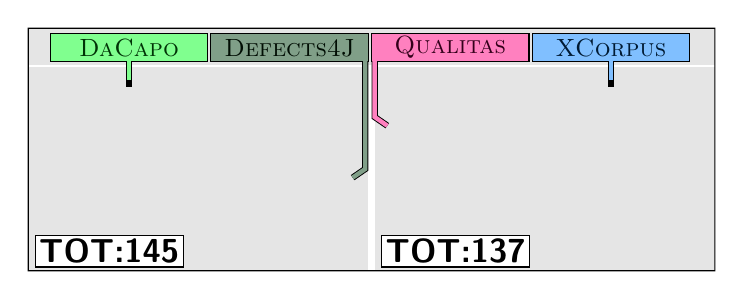
\begin{tikzpicture}[xscale=0.8, yscale=0.55,
    venncellstyle/.style={fill=white, inner sep=1.2pt, rounded corners=1, minimum width=0.6cm, minimum height=0.45cm},
    venncellstylebg/.style={fill=black, opacity=0.5, inner sep=1.2pt, rounded corners=1, minimum width=0.6cm, minimum height=0.45cm},
      vennfill/.style={rounded corners=4, opacity=0.5},
      venndraw/.style={rounded corners=4, black, thick, opacity=0.8},
      legend/.style={draw, rounded corners=0, minimum height=0.35cm, minimum width=2cm, inner sep=0},
      every text node part/.style={align=center}
  ]

  % Draw the background for the legend connectors
  \begin{scope}[xshift=0.25cm, yshift=0.3cm]
    \draw[line width=0.08cm, -, black]
    	(1.25, 0.1) -- ++(0, -0.6);
    %% \draw[line width=0.08cm, -, black]
    %% 	(4.8, 0.1) -- (5, -1.5) -- (5, -2.9) -- (4.8, -3.1);
    %% \draw[line width=0.08cm, -, black]
    %%     (5.35, 0.1) -- (5.15, -0.5) -- (5.15, -1.2) -- (5.35, -1.4);
    \draw[line width=0.08cm, -, black]
	(5, 0.1) -- (5, -1.5) -- (5, -2.4) -- (4.8, -2.6);
    \draw[line width=0.08cm, -, black]
        (5.15, 0.1) -- (5.15, -0.5) -- (5.15, -1.2) -- (5.35, -1.4);
    \draw[line width=0.08cm, -, black]
        (8.9, 0.1) -- ++(0, -0.6);
  \end{scope}

  % For each benchmark
  \foreach \benchname/\x/\y/\results in { % individual venn intersection numbers are {x/y/count/percentage}
		TOT:145/0/0/{    4/-3/16/100, 4/-1/42/100,  3/-1/66/100, 2/-1/4/100, 3/0/6/100, 1/0/11/100},
		TOT:137/5.5/0/{       3/-3/1/100,4/-3/14/100, 4/-1/39/100,  3/-1/64/100,3/-2/1/100, 2/-1/6/100, 3/0/3/100, 1/0/6/100, 1/-1/2/100,2/0/1/100}}
  {
    % shift figure to the right coordinates
    \begin{scope}[xshift=\x cm, yshift=\y cm]

    \fill[black, opacity=0.1] (-0.1,0.25) rectangle (5.3,-4.45);

    % First draw transparent fill, then draw hard boundaries w/o transparency
    \foreach \styledraw in {\Xclear, \Xfilldraw}{ % , \Xdash
      % % SonarQube
      \styledraw{(2, 0.2) rectangle (4, -4.2)}{SQ}{dash pattern=on 0.5pt off 0.5pt};
      % % JJI
      \styledraw{(0, -1) rectangle (5, -3)}{JJI}{dash pattern=on 0.4pt off 1pt};
      % IntraJ-N
      \styledraw{(1, 0) rectangle (3, -4.4)}{IJH}{dash pattern=on 0.4pt off 3pt};
      % IntraJ-NN
      \styledraw{(0.2, -2) rectangle (5.2, -4)}{IJnonH}{black};
    }

    % Draw the individual markers
    \foreach \vennx/\venny/\count/\percent in \results {
      \venncell[\percent]{\vennx, \venny}{\count};
    }

    % Draw benchmark name
       % Draw benchmark name
    \node at (0, -4.)
          [right, draw, fill=white, minimum height=0.4cm, inner sep=1.5pt] {\textbf{\large \textsf{\benchname}}};
    {}

    \end{scope}
  }

  \fill[opacity=0.1] (-0.1,0.3) rectangle (10.8, 1.15);

  % Draw the legend
  \begin{scope}[xshift=0.25cm, yshift=0.3cm]

    \node at (1.25, 0.4)
          (IJH)
          [legend, fill=white!50!IJH] {\textcolor{black!80!IJH}{{\small \tool{DaCapo}}}};

    \node at (3.80, 0.4)
          (IJnonH)
          [legend, fill=white!50!IJnonH] {\textcolor{black!80!IJnonH}{{\small \tool{Defects4J}}}};

    \node at (6.35, 0.4)
          (JJI)
          [legend, fill=white!50!JJI] {\textcolor{black!80!JJI}{{\small \tool{Qualitas}}}};

    \node at (8.9, 0.4)
          (SQ)
          [legend, fill=white!50!SQ] {\textcolor{black!80!SQ}{{\small \tool{XCorpus}}}};

    {}
    % Manual coordinates to syncronise with the background color bit from before all else is drawn
    \draw[ultra thick, -, white!50!IJH]
    	(1.25, 0.15) -- ++(0, -0.5);
    %% \draw[ultra thick, -, white!50!IJnonH]
    %% 	(4.8, 0.1) -- (5, -1.5) -- (5, -2.9) -- (4.8, -3.1);
    %% \draw[ultra thick, -, white!50!JJI]
    %%     (5.35, 0.1) -- (5.15, -0.5) -- (5.15, -1.2) -- (5.35, -1.4);
    \draw[ultra thick, -, white!50!IJnonH]
	(5, 0.15) -- (5, -1.5) -- (5, -2.4) -- (4.8, -2.6);
    \draw[ultra thick, -, white!50!JJI]
        (5.15, 0.15) -- (5.15, -0.5) -- (5.15, -1.2) -- (5.35, -1.4);
    \draw[ultra thick, -, white!50!SQ]
        (8.9, 0.15) -- ++(0, -0.5);

  \end{scope}

  % top label


  %% bounding box
  \draw (current bounding box.north east) -- (current bounding box.north west) -- (current bounding box.south west) -- (current bounding box.south east) -- cycle;

\end{tikzpicture}

\caption{\label{fig:corporaOverlap} Project overlap. In the left diagram, two projects with the same name but different versions are counted as distinct---the diagram to the right shows overlap when versions are disregarded.}
\end{figure}
Figure~\ref{fig:corporaOverlap} shows the overlap between the four corpora as two Venn diagrams where each number represents a project. In the left diagram,  two versions of the same project are counted as two separate projects. In the right diagram, we only consider the project name, disregarding the version.
From the left diagram, we can see that Defects4J does not overlap with any other corpus analysed. As expected, most of the projects are shared across Qualitas and XCorpus as XCorpus was built as an extension of Qualitas. From the diagrams, we can see that eight projects (145-137) are used among the corpora, but with different versions. Table~\ref{tbl:sameprojects} details these projects and versions.

% \usepackage{multirow}
% \usepackage{booktabs}



\subsubsection*{\textbf{Discussion}}
Table~\ref{tbl:corpusAnalysis} provides insight into the features utilised by each project. Using Qualitas Corpus as an illustration, we see that \code{strictfp} is only used in four projects.
Similarly, in DaCapo, fewer than fifty percent of the projects use concurrency libraries.
With JFeature, we can achieve a fine-grained classification of the properties. We can, for instance, distinguish between uses and declarations of annotations, and when it comes to generics, we can distinguish between the declarations of generic methods, classes, and interfaces, providing the user with a better comprehension of the corpus.
It is apparent that most projects utilise only Java 4 and Java 5 features. With the exception of Defects4J, few projects employ Java 7 and Java 8.
Indeed, this table reveals that Defects4J is the most modern corpus, as nine of the fourteen assessed applications utilise at least one of the observed Java 8 features.




\section{Extensibility}
\label{sec:extension}
Extensibility is one of the key characteristics of JFeature. Users can create new queries to extract additional features, making use of all attributes available in the ExtendJ compiler.
We illustrate this by adding a new feature, \textsc{Overloading}, that measures the number of overloaded methods in the source code.
Listing~\ref{lst:overloading} shows the JastAdd code for this: we define a new boolean attribute, \code{isOverloading}, that checks if a method is overloaded. We then use this attribute to conditionally contribute to the \code{features} collection, only for overloaded method declarations.
The attribute \code{isOverloading} is defined using several ExtendJ attributes:
the attribute \code{hostType} is a reference to the enclosing type declaration of the method declaration.
A type declaration, in turn, has an attribute \code{methodsNameMap} that holds references to all methods for that type declaration, both local and inherited. If there is more than one method for a certain name, that name is overloaded.

\begin{lstlisting}[language=JastAdd, numbers=none, label=lst:overloading ,caption=Definition of the \textsc{Overloading} feature]
MethodDecl contributes
  new Feature("JAVA1", "Overloading", getCU().path())
  when isOverloading() to Program.features();

syn boolean MethodDecl.isOverloading()
  = hostType().methodsNameMap().get(getID()).size() > 1;
\end{lstlisting}
For the computation to work, it is necessary to supply the classpath, so that ExtendJ can find the classfiles for any direct or indirect supertypes of types in the analysed source code.
We analysed 16 distinct projects for which we  successfully extracted the classpaths and dependencies required for ExtendJ compilation. The results provided by JFeature for the sixteen projects are summarised in Table~\ref{tbl:overloading}. As can be seen, each project has overloaded methods. In some cases, such as \code{commons-codec}, \code{commons-math}, and \code{ jackson-core}, more than one fifth of the methods are overloaded.

\textsc{Overloading} is a good example of a feature that requires semantic analysis---it can not be computed by a simple pattern match using regular expressions or a context-free grammar.

\begin{table}[]
\centering
\setlength\tabcolsep{3pt}
\begin{tabular}{|l|r|r|r|r|}
\hline
\multicolumn{1}{|c|}{\textsc{Projects}} & \multicolumn{1}{c|}{\textsc{$\sim$ KLOC}} & \multicolumn{1}{c|}{\begin{tabular}[c]{@{}c@{}}\textsc{Number}\\of \textsc{Methods}\end{tabular}} & \multicolumn{1}{c|}{\begin{tabular}[c]{@{}c@{}}\textsc{Overloaded}\\\textsc{Methods}\end{tabular}} & \multicolumn{1}{c|}{\%}  \\
\hhline{|=====|}
antlr-2.7.2      & 34  & 2081 & 358        & 17,2          \\
\hline
commons-cli-1.5.0          &  6  & 585  & 76         & 13 \\
\hline
commons-codec-1.16-rc1     &  24  & 1812 & 422        & 23,3          \\
\hline
commons-compress-1.21     &  71   & 5359 & 571        & 10,7          \\
\hline
commons-csv-1.90           & 8   & 716  & 93         & 13 \\
\hline
commons-jxpath-1.13       &   24  & 2030 & 167        & 8,23          \\
\hline
commons-math-3.6.1       &   100   & 7229 & 1779       & 24,6          \\
\hline
fop-0.95       &   102  & 8317 & 666        & 8,01          \\
\hline
gson-2.90   &     25   & 2289 & 125        & 5,46          \\
\hline
jackson-core-2.13.2    &    48    & 3687 & 839        & 22,8          \\
\hline
jackson-dataformat-2.13   &  15   & 1122 & 161        & 14,3          \\
\hline
jfreechart-1.0.0         &   95   & 6980 & 1000       & 14,3          \\
\hline
joda-time-2.10           &  86    & 9324 & 1257       & 13,5          \\
\hline
jsoup-1.14      &  25  & 2556 & 408        & 16 \\
\hline
mockito-4.5.1 &   19   & 2054 & 318        & 15,5          \\
\hline
pmd-4.2.5     &   60   & 5324 & 1021       & 19,2          \\
\hline
\end{tabular}
\caption{\label{tbl:overloading} Results from the \textsc{Overloading} feature.}
\end{table}


\section{Use cases for JFeature}
\label{sec:discussion}
We already discussed two possible use cases for JFeature: corpus evaluation (Section~\ref{sec:corpora}), and extending JFeature to identify specific features (Section~\ref{sec:extension}). In this section, we discuss two additional use cases: longitudinal studies and project mining.
\subsection{Longitudinal Study}
JFeature can be used to conduct longitudinal studies, i.e., changes occurring over time. As an example, we conducted a study on Mockito and its evolution on the adaption of Java 8 features over time. Mockito is one of the most popular Java mocking frameworks and has an extensive history with over 5,000 commits. Java 6 was utilised by Mockito until version 2.9.x. With version 3.0.0, Java 8 was adopted.
\begin{figure}[b]
\begin{subfigure}{.5\columnwidth}
  \centering
  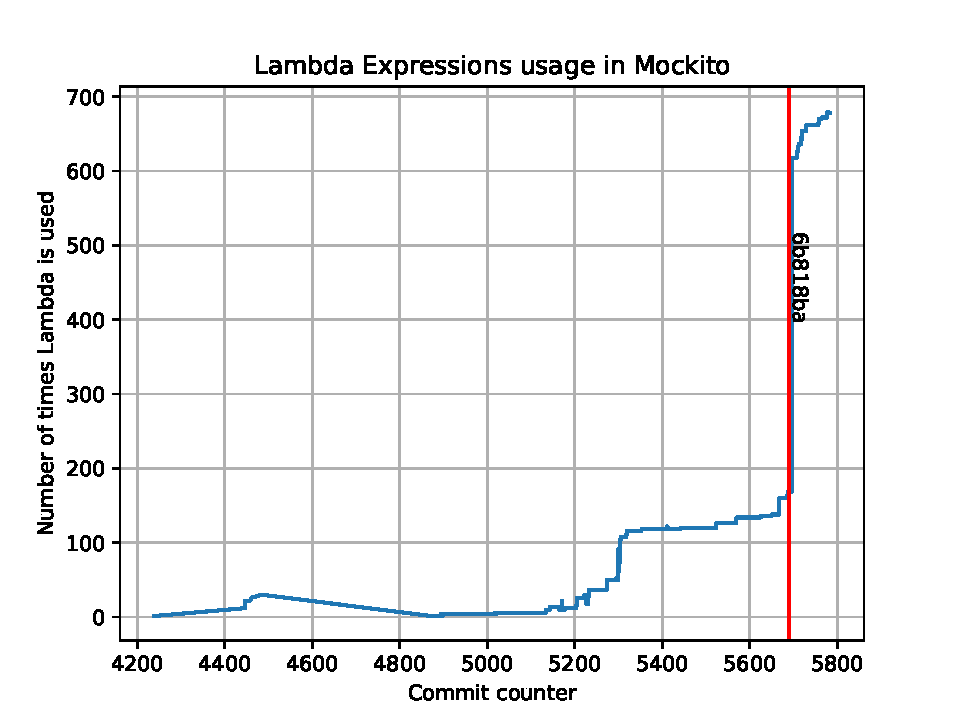
\includegraphics[width=1.\linewidth]{papers/jfeature/img/lambda_count.pdf}
\end{subfigure}%
\begin{subfigure}{.5\columnwidth}
  \centering
  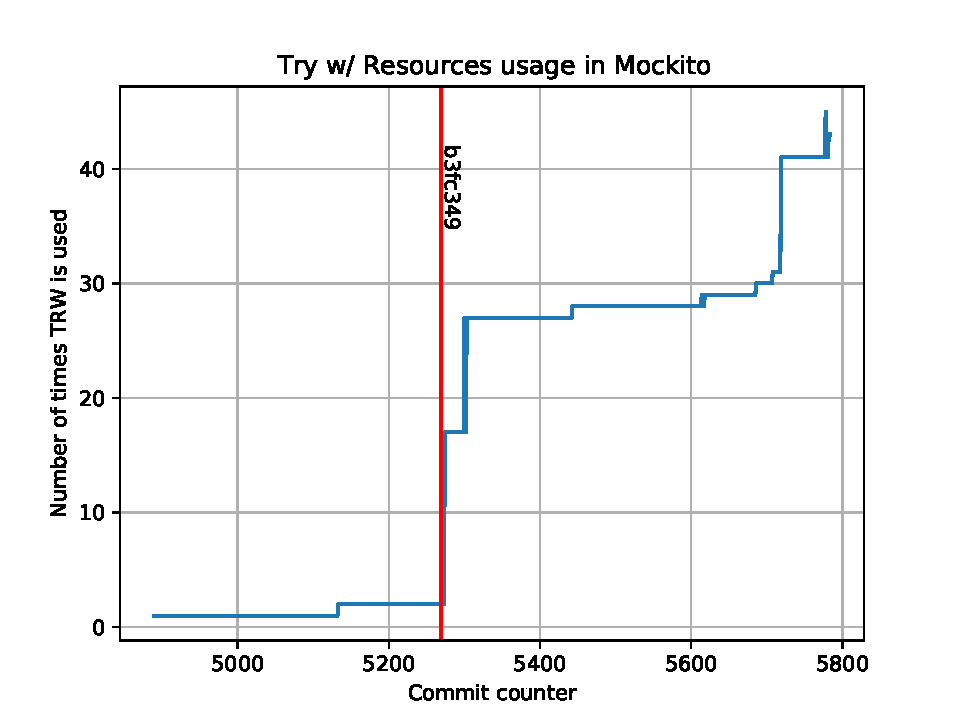
\includegraphics[width=1.\linewidth]{papers/jfeature/img/TWR_count.pdf}
\end{subfigure}%
\caption{\label{lbl:mockito} Usage of \textsc{Lambda Expressions} and \textsc{Try With Resources} in Mockito over time.}
\end{figure}
The evolution of the occurrences of \textsc{Lambda Expressions} and \textsc{Try With Resources} is depicted in Figure~\ref{lbl:mockito}. As can be seen, at commit number 5269\footnote{Commit: b3fc349.}, there is a substantial increase in utilisation of try with resources, whereas at commit number 5696\footnote{Commit: 6b818ba.}, there is a significant increase in the use of lambda expressions.

\subsection{Project mining}
Contemporary revision control hosting services (GitHub\footnote{\url{https://github.com}}, GitLab\footnote{\url{https://gitlab.com}}, bitbucket\footnote{\url{https://bitbucket.org}}) offer uniform interfaces to the source code of millions of software projects.
These interfaces enable researchers to ``mine'' software projects at scale, filtering by certain predefined properties (e.g., the number of users following the project or the main programming language).
For example, the \textit{GitHub Java Corpus}~\cite{githubCorpus2013} collects almost 15,000 projects from GitHub, filtered to only include Java projects that have been forked at least once.
Combining JFeature with these query mechanisms allows researchers to select projects by more detailed syntactic and semantic features.
For instance, a corpus suitable for answering questions about race detection~\cite{li2014rfbi}
could select projects that make explicit use of \textsc{java.util.concurrent.*},
while an exploration of functional programming patterns~\cite{cok2018reasoning} could select projects that use \textsc{Lambda Expressions} and \textsc{Method References}.


\section{Related work}
\label{sec:related-works}
Existing tools for code metrics are usually focused on code quality metrics, rather than what language features are used, and typically analyse the intermediate representation rather than the source code. One example is the CKJM tool~\cite{Spi05g} for the Chidamber and Kemerer metrics~\cite{chidamber1994metrics}. Another example, that more closely resembles ours, is jCT, an extensible metrics extractor for Java 6 IL-Bytecode, introduced by Lumpe et al.~\cite{jCT}, in 2011.
Like us, they evaluated their tool on Qualitas Corpus; however, because jCT works only on annotated bytecode and not on
source code, the number of features that can be extracted is limited.
A significant amount of information is lost during the compilation of Java source code to Java bytecode.
For example, enhanced \code{for} statements, diamond operators and certain annotations, such as \code{@Override}, are not present in the bytecode.
For XCorpus, the authors analysed the language features used, and a summary was presented in their paper~\cite{dietrich2017xcorpus}.
They also analysed the bytecode, which was implemented using the visitor pattern.


%In~\cite{dietrich2017xcorpus}, Dietrich et al. analyze the present a summary of the features of XCorpus programmes similar to ours, but computed using scripts over the bytecode.
%REMOVED THIS SENTENCE because they say the scripts are available./GH
%This provides the user with an overview of the corpus, but the user will be unable to analyse a subset of the projects in the corpus.

A way to improve the user experience would be to integrate JFeature with a visualisation tool like \textit{Explora}~\cite{merino2015explora}. The idea
behind \textit{Explora} is to provide to the user a visualisation tool designed for simultaneous analysis of multiple metrics in software corpora.
Finally, JFeature may be enhanced by incorporating automated dependency extractors, such as MagpieBridge's \emph{JavaProjectService}~\cite{luo_et_al:LIPIcs:2019:10813}, to infer and download libraries automatically. Currently, JavaProjectService infers the dependencies for projects using \emph{Gradle} or \emph{Maven} as build system.





\section{Conclusions}
\label{sec:conclusions}
We have presented JFeature, a declarative and extensible static analysis tool for the Java programming language that extracts syntactic and semantic features.
JFeature comes with twenty-six predefined queries and can be easily extended with new
ones.

We ran JFeature on four widely used corpora: the DaCapo Benchmark Suite, Defects4J, Qualitas Corpus, and XCorpus.
We have seen that, among  the corpora, Java 1-5 features are predominant. This leads us to conclude that some of the corpora may be less suited for the evaluation of tools that address features in Java 7 and 8.

We have illustrated how JFeature can be extended to capture semantically complex features by writing the queries as attribute grammars, extending a full Java compiler. This allows powerful queries to be written that can make use of all the compile-time properties computed by the compiler.

We discussed several possible use cases for JFeature: evaluation of corpora, mining software collections to create new corpora, and longitudinal studies of how projects have evolved with regard to the use of language features.
We also note that for some features to be analysed, the full classpath and dependencies are required. An interesting future direction is therefore to combine JFeature with recent tools that support automatic extraction of such information from projects that follow common build conventions.


%\newpage
% \bibliographystyle{abbrv}
% \bibliography{bibliography}







% \end{document}
% \endinput
